\documentclass{article}
\usepackage{filecontents}
\usepackage[left=2.5cm,top=2.5cm,right=2.5cm,bottom=2.5cm]{geometry}
\usepackage{amsmath}
\usepackage{array}
\usepackage{caption}
\usepackage{placeins}
\usepackage{graphicx}
\usepackage{subcaption}
\usepackage{setspace}
\usepackage{animate}
%\usepackage[active,tightpage]{preview}
\usepackage{natbib}
\bibpunct{(}{)}{,}{a}{}{;} 
\usepackage{url}
\usepackage{nth}
\usepackage{authblk}
\usepackage{listings}
% for the d in integrals
\newcommand{\dd}{\; \mathrm{d}}
\newcommand{\tc}{\quad\quad\text{,}}
\newcommand{\tp}{\quad\quad\text{.}}
\bibliographystyle{apalike}

\title{Homicide, health, and deviations from best practices mortality: Mortality in Mexican states, 1990-2010}

\author[1]{Jose Manuel Aburto\thanks{aburtoflores@demogr.mpg.de}}
\author[2]{Tim Riffe}
\affil[1]{Max Planck Institute for Demographic Research, EDSD}
\affil[2]{Max Planck Institute for Demographic Research}


\begin{document}

\maketitle

\begin{abstract}
We analyze trends in temporary life expectancy for three large age groups from 1990 to 2010 for all 32 Mexican states, and compare these with a synthetic best practices trend. We assess the impact of amenable/avoidable mortality on temporary life expectancy at the state level by sex. We apply demographic measures and use standard decomposition techniques to disentangle the effects of selected causes of death. We find improvements in temporary life expectancy for the population aged 0 to 14, as they continuously approached the best practices trend. However, the adult population aged 15 to 39 shows deterioration among males after 2006 in almost every state. Opposing this trend, females show a convergence trend toward the best practices benchmark between ages 15 and 39. Adults aged 40 to 74 show an unexpected decrease in the best practices indicator, and major variation among states in temporary life expectancy. These findings might strengthen the case for reforms that will enable all the Mexicans to improve in their health status.
​



\end{abstract}


\section*{Background}
The \nth{20} century was marked by sizable improvements in mortality, living
conditions and health in most Latin American countries \citep{who2000}. In
Mexico, these improvements have slowed down recently as a result of opposing
trends in particular causes of death. For instance, homicide and diabetes
increased drammatically, even as infectious and
respiratory diseases continued to fall. While life
expectancy at birth increased by 4.3 years for males (from 67.6 to 71.9) and 3.4
for females (from 73.8 to 77.2) between 1990 and 2000 \citep{SOMEDE},
between 2000 and 2010, life expectancy at birth entered into a period of
stagnation for males and slowed progress for females \citep{canudas2014}. This
period coincides with the implementation of different public health
interventions, such as the Universal Vaccination Program and Seguro
Popular, which aim to provide primary and secondary
health care to the uninsured population, allocate funds to cover catastrophic
health expenditures \citep{knaul2005}. Further, the Oportunidades program
was introduced to supply incentives for families to invest in themselves and
benefit from education, health, and nutrition \citep{neufeld2012}. Some evidence
suggests that Mexico experienced substantial decreases in infant and child
mortality, along with improvements that contributed to the reduction of
mortality and in the prevalence of acute malnutrition between 1980 and 2000
because of these interventions \citep{sepulveda2006}. Similarly, some evidence
suggests that by 2012 Seguro Popular had covered an additional 52 million
people in Mexico that did not have any access to public health care and, as a result, there has been a reduction in catastrophic health expenditures \citep{knaul2012}.

 Although these results are important, they do not reveal heterogeneity between
 Mexican states, which is an important task given the high degree of social and
 health inequalities in Mexico and the heterogeneity in how public health interventions have taken place within the states (e.g., Oportunidades is focused on the poorest states and Seguro Popular did not started at the same time in the states) \citep{Frenk2006}.  Given these improvements
 in health care coverage, the strong role of institutions, and ongoing public
 health interventions, it is necessary to assess the varied impacts that
 these health interventions may have had on particular causes of death in states
 populations and across the country.
 
 One approach to assess the impact of health services is by operationalizing the
 concept of Avoidable/Amenable Mortality (hereafter abbreviated AM)
 \citep{nolte&mckee2004, nolte&mckee2008}. This construct aims to measure the quality of health service systems by selecting certain
 causes of death that should not occur in the presence of effective and
 timely health care. Among industrialized countries (e.g., United States,
 Australia, France, Japan), a reduction in AM rates was
 observed from the late 1990's into the \nth{21} Century
 \citep{nolte&mckee2008}. Avoidable mortality rates fell, on average, by 17\%
 for males and 14\% for females in these countries. Despite mortality reductions for
 both sexes, heterogeneity between countries was identified, with the United
 States showing the smallest reductions (around 5\%) for both sexes. However,
 each country showed progress in mortality from treatable cancers and
 circulatory diseases except for ischemic heart diseases.

In Mexico, the components of avoidable mortality had different trends since the
late 1990's. Between 2000 and 2004 AM decreased, particularly from
infectious diseases and nutrition-related conditions \citep{francomarina2006}, while it increased between 1998 and 2010 due to diabetes, circulatory diseases, perinatal and respiratory conditions
\citep{agudelo2014efecto}. Increases in the latter causes
of death were particularly concentrated in the poorest states of the country
\citep{davila2014mortalidad}. We aim to improve on these studies
by a more focused segmentation of AM into health intervention-related AM and
behavior-related AM. Also, we extend analysis to all 32 states, by sex, and over
the full 21-year period from 1990 to 2010.\footnote{In the final revision of
this paper we will provide series through 2013. Right now the exposures are not
yet prepared for years after 2010.} Finally, we compare state mortality patterns
with best-practice benchmarks for large age groups (e.g., 0-14, 15-39, 40-75). These best practice
benchmarks are calculated on the basis of the lowest observed mortality within
ages and causes, among the full set of 32 Mexican states. This concept was first
proposed by \citet{wunsch1975minimum}, later explored by
\citet{vallin2008minimum}, and more recently applied under a different
definition by \citet{eikemo2014}. We apply demographic measures and
standard decomposition techniques to isolate the cause and age-specific shortcomings between states and the corresponding best-practices lifetable. 

We hypothesize age-dependent variations in temporary life expectancy outcomes.
In particular, we expect convergence between states in temporary life expectancy
for young people, since public health interventions are mainly focused in infant
mortality and child health. For instance, the vaccination program and the health
reform aim to fully cover children in the entire country, and recent
evidence suggests a decrease in mortality between ages 0 to 14 due to a decline
in infectious and respiratory diseases \citep{canudas2014}. On the contrary, we
expect little improvements in temporary life expectancy for the adult and older
adult population due to the unprecedented rise in homicide mortality and the
increase in diabetes mortality in these ages \citep{canudas2014}. Although every
state has the commitment to providing universal coverage and equitable access to
health care since the early 2000's, we anticipate heterogeneity between states
in mortality improvements due to state differences in epidemiological patterns
\citep{Frenk2006}.


\section*{Data \& Methods} 
 
We used death counts available from official microdata files produced by the
Mexican Statistical Office from 1990 to 2010 \citep{INEGI}. These data contain
information on causes of death by single age, sex, and place of residence at the
time of death. In addition, we used population estimates (Exposures) corrected
for age misstatement, undercounting, and migration--- both internal and
international--- available from the Mexican Society of Demography to construct
cause-age-specific death rates by sex and state from 1990 to 2010 \citep{SOMEDE}.

\subsection*{Classification of Causes of Death}

To separate causes of death that are susceptible to medical intervention (e.g.,
infectious and respiratory diseases) and those related to health behaviors and
intersectoral policies (e.g., homicides, lung cancer) we use the concept of
'Amenable/Avoidable Mortality' (AM) \citep{nolte&mckee2004, nolte&mckee2008}. This
concept assumes a list of conditions that should not occur with the availability
of timely medical care. Recently, this concept has also been used to gauge the
effect of causes that can be influenced by public policy (e.g., cirrhosis) \citep{elo2014}. We classified causes of death into ten groups based on prior studies
\citep{elo2014, Aburto2015}, as listed in Table~\ref{tab:causes}, with
relative frequencies by sex.

% latex table generated in R 3.1.2 by xtable 1.7-4 package
% Wed Sep 23 21:57:18 2015
\begin{table}[ht]
\centering
\caption{Avoidable Mortality classification, with crude percentages below age 75.}
\label{tab:causes}
\begin{tabular}{>{\raggedright}m{3cm}rr}
Group/Cause  & Males & Females \\ 
  \hline
Causes amenable to medical service & 28.50 & 40.24 \\ 
  Diabetes & 9.07 & 14.77 \\ 
  Ischemic heart diseases & 7.92 & 6.66 \\ 
  HIV/AIDS & 1.80 & 0.51 \\ 
  Lung cancer & 1.58 & 1.09 \\ 
  Cirrhosis & 5.34 & 1.09 \\ 
  Homicide & 5.95 & 1.05 \\ 
  Road traffic accidents & 5.82 & 2.26 \\ 
  Suicide & 1.48 & 0.46 \\ 
  Other causes & 32.53 & 31.86 \\ 
   \hline
\end{tabular}
\end{table}

We separate diabetes, ischemic heart diseases (IHD), HIV/AIDS, lung
cancer, and cirrhosis because all of them are amenable to both health behavior
and medical service, and because the first two represent major causes of death
in Mexico \citep{canudas2014}. In addition to these causes, we also isolate
homicide, road traffic accidents, and suicide because they have emerged as
leading causes of death among young people, and the first two had a sizeable
impact on life expectancy recently in Mexico \citep{canudas2014}. All causes of death were classified using the International Classification of Diseases, revision 9 for the period 1990-1997 and the tenth revision for 1998-2010 (see Apppendix Table 1 for details on ICD codes for each cause).

We truncated analysis at age 75 because classification of causes of deaths and age reporting are considered to be innacurate in death registration at older ages \citep{tobias2001} and because most changes in life expectancy are likely due to changes in mortality patterns below the age of 75 \citep{Aburto2015}. In addition, health care and policy/behavior interventions are more likely to be effective at younger ages \cite{elo2014}.


\subsection*{Demographic Methods}
We first smooth cause-specific death rates over age and time for each
state and sex separately using the 2-d p-spline method proposed by
\citet{GC2012}.
This helps eliminate stochastic zeros, which otherwise would accumulate in the best-practices mortality
schedule, and artificially inflate BP life expectancy. Smoothed death rates are
then constrained to sum to the unsmoothed all-cause death rates. There are no
zeros in all-cause death rates. We then calculate period life tables up to
age 74 for males and females from 1990 to 2010 following the HMD Methods
Protocol \citep{HMDMP}. Second, we estimated temporary life expectancy to
capture differential effects of all-cause mortality among three large age
groups: children (ages 0-14), young adults (ages 15-40) and older adults
(40-74). We do this following the formulas of \citet{arriaga1984}, as
defined below.

We then construct the best practices lifetables (BP) for every year and sex
and estimated cause-specific contributions to the difference between
state-specific temporary life expectancy and BP temporary life expectancy
($e^{\star}$) applying standard decomposition methods
\citep{horiuchi2008}.\footnote{The decomposition will be carried out and
incorporated in the final paper version.} All the analyses were carried out
using \texttt{R}.

\subsection*{Best Practices Lifetable}
This approach was first proposed by \citet{wunsch1975minimum}, and we summarize it
briefly here. The synthetic best practices (BP) lifetable is a composite of the
lowest observed mortality rates by age, cause, and state for a given sex and year. In continuous terms, we define life expectancy, $e(0)$, as:
\begin{equation}
\int _0 ^\infty l(x) \dd x \tc
\end{equation}
where $l(x)$ is the survivorship function defined with radix of one, or as a
function of the force of mortality, $\mu(x)$ as:
\begin{equation}
\label{eq:lx}
l(x) = e^{-\int_0^x \mu(a) \dd a}
\end{equation}

In general, $\mu(x)$ can be treated as the sum of $I$ cause-specific mortality
rates at age $x$ assuming that causes of death are independent of one another:
\begin{equation}
\label{eq:mxmin}
\mu(x)^{\star} = \sum_1^I min(\mu_i(x))
\end{equation}
This BP mortality rate schedule ($\mu^{\star}(x)$) has a unique
age profile, and it determines a pattern of $l(x)^{\star}$, per \eqref{eq:lx}, that corresponds with a
best practices life expectancy, $e(0)^{\star}$. Thus, $e(0)^{\star}$ can be treated as a
maximum presently achievable life expectancy given the best available
practices and technologies within a given set of populations and assuming
perfect diffusion \citep{vallin2008minimum}. It is an imaginary quantity because no particular population
ever achieves this mortality pattern, and none may ever. However, this value is
a real referent not based on a projection of improvements into the future, and
so it bounds our optimism in a practical way. This definition of best practices
is different from other uses found in the literature, and it is important to
notice that it is not the same as the vanguard, or record-holder life
expectancy. Vanguard life expectancy is the notion that was treated by
\citet{oeppen2002broken}, and it is different from our definition of best
practices in that the vanguard life expectancy of a given year is based on
all-cause mortality and refers to a single population.

\subsection*{Temporary Life Expectancy}

We require an estimate of temporary life expectancy between ages
$x_1$ and $x_2$, for $x_1<x_2$, or the average years of life lived between these ages according to a given set of period mortality rates \citep{arriaga1984}. We denote this quantity as
$e(x_1,x_2)$, and its best practices maximum as $e^{\star}(x_1,x_2)$. Defined in
terms of $l(x)^\star$:

\begin{equation}
e^{\star}(x_1,x_2) = \frac{\int _{x_1}^{x_2} l(x)^\star \dd x}{l(x_1)^\star}
\end{equation}

\subsection*{Limitations}
The limitations of our study should be mentioned. First, mortality data are
likely to present innacuracies in cause-of-death classification due to
comorbidities, particularly at older ages \citep{tobias2001}. To mitigate this,
we focus on ages below 75, grouping causes of death using ICD codes according to
the avoidable mortality concept.
Second, our estimates regarding homicide mortality are likely to be
underestimated because of inaccurate practices regarding counting, reporting,
and due to the large number of missing individuals in Mexico \citep{HRW2011}.
Third, avoidable mortality should be understood as an indicator of potential
weaknesses with respect to health care and some public health policies and not
as a definitive assessment \citep{nolte&mckee2008}. Fourth, the amount of deaths
that should be considered avoidable within the avoidable classification is not
clear \citep{beltran2011avoidable}. For instance, \citet{nolte2012amenable}
consider only 50 percent of heart disease amenable in industrialized countries,
based on a previous review of evidence.

We do not have information to precisely
measure percentages of avoidable mortality within cause groups. Nonetheless, the
difference between a given mortality schedule and the best practices schedule of
the same year can be conceived of as a minimal definition of avoidable
mortality, a sort of lower bound to how much mortality could have been avoided.
Certainly, even a best practices schedule will contain elements of mortality
most would consider avoidable. To the extent that the components of the BP schedule were indeed
attained somewhere in the popualtion universe, one can view any excess mortality
with respect to the BP schedule as avoidable. The concept of BP is nonetheless a
model, and not a real population, but we find it useful. Since we conduct
age-cause decompositions against the BP trend in each year, we consider both
views of avoidability.

Despite limitations in data, we made use of the most reliable data available
publicly to perform our analyses at the sub-national level in Mexico accounting
for all the cause codes required for this study.

\section*{Results}
\subsection*{Trends in best practices life expectancy}

Figure 1 shows state-specific  (black lines), vanguard  (red lines) and BP (blue
lines) remaining life expectancies for ages 0-14 (\ref{fig:e0_14} ), 15-39
(\ref{fig:e15_39}) and 40-74 (\ref{fig:e40_74}). The red line represents the
vanguard life expectancy out of the 32 states within each year and the blue line
represents the maximum potentially achievable for the Mexican population under
the best practices definition.
The figures clearly shows a convergence pattern among the states toward the BP
expectancy through at least the year 2000; however the latter period shows
stagnation and even decreases for some states.

\begin{figure}
\centering
\caption{Temporary life expectancy for states (black line), vanguard life
expectancy (red) and best practices life expectancy by sex, 1990-2010.}
\begin{subfigure}{\textwidth}
\centering
\caption{$e(0,14)$}
\vspace{-2em}
\label{fig:e0_14}
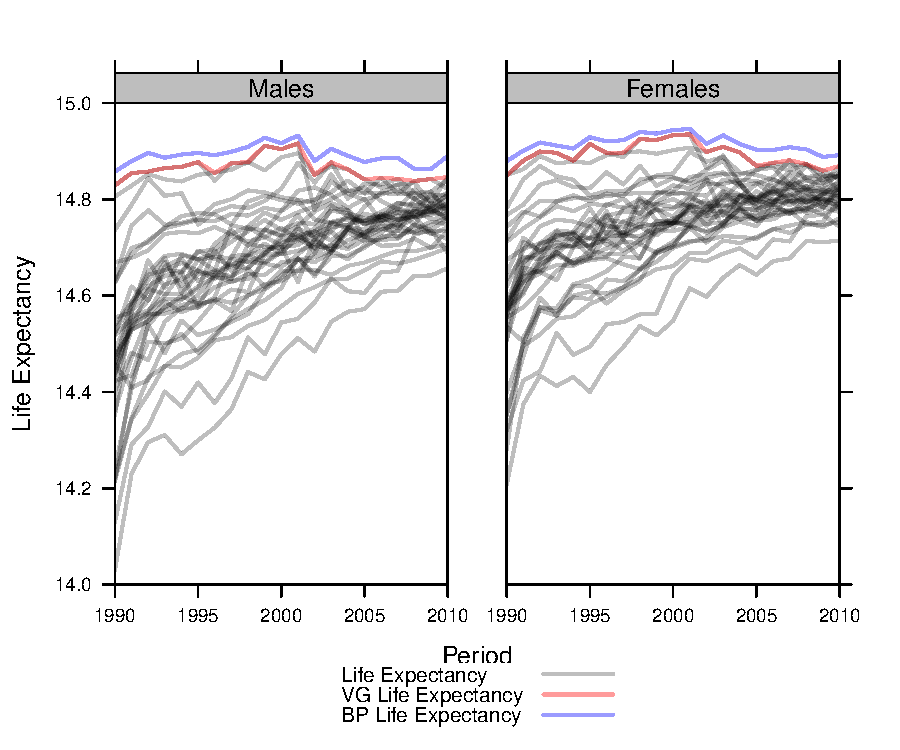
\includegraphics[scale=.5]{Figures/et0_14.pdf}
\end{subfigure}
\\
\begin{subfigure}{\textwidth}
\centering
\caption{$e(15,39)$}
\vspace{-2em}
\label{fig:e15_39}
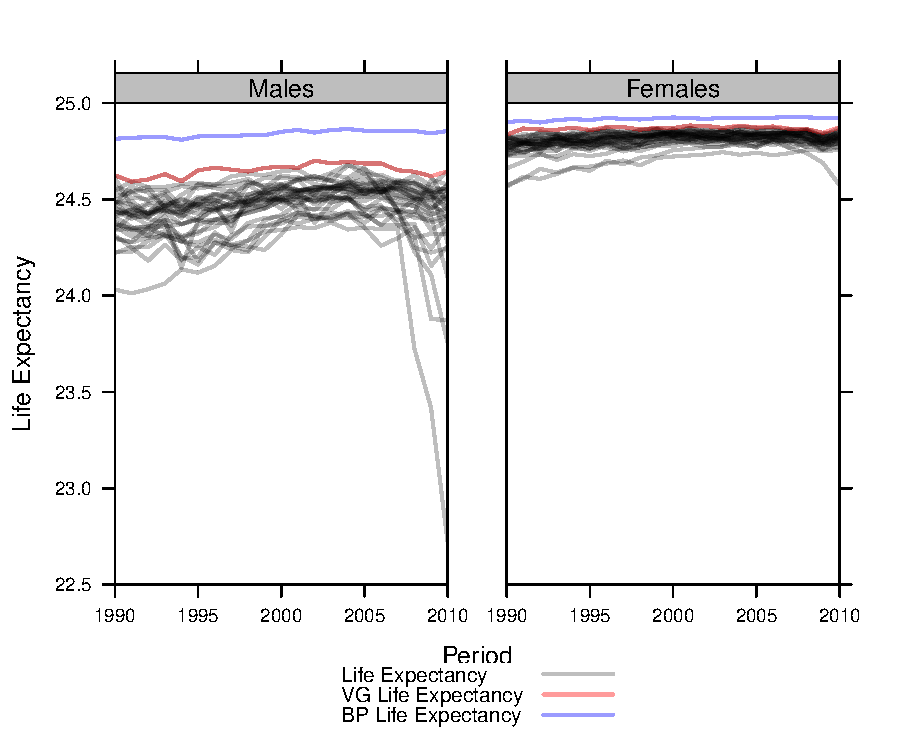
\includegraphics[scale=.5]{Figures/et15_39.pdf}
\end{subfigure}
\\
\begin{subfigure}{\textwidth}
\centering
\caption{$e(40,74)$}
\vspace{-2em}
\label{fig:e40_74}
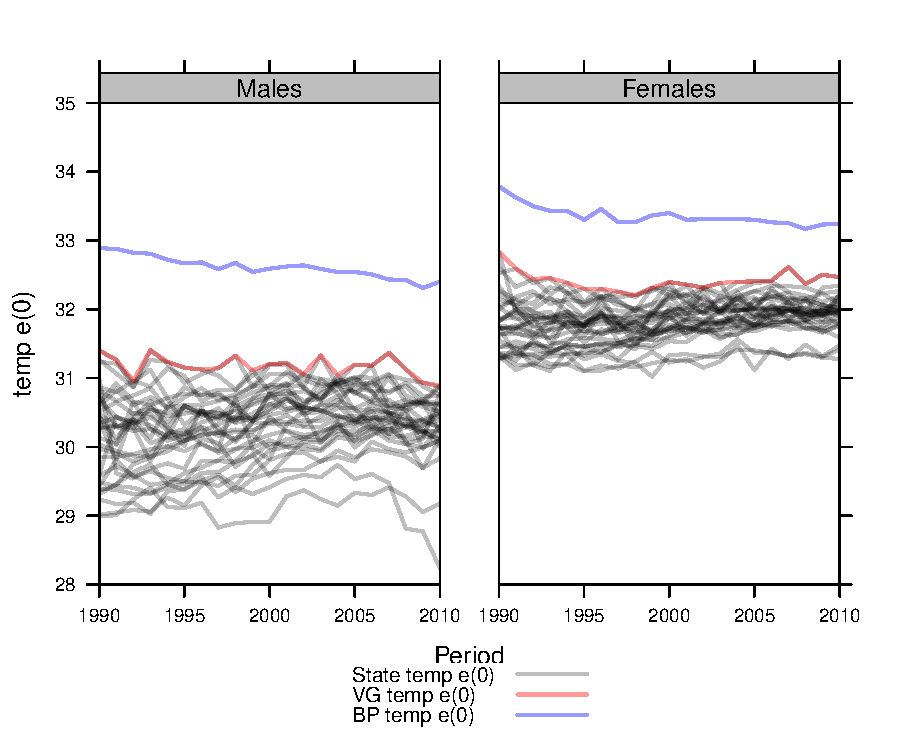
\includegraphics[scale=.5]{Figures/et40_74.pdf}
\end{subfigure}
Source: own calculations based on INEGI and SOMEDE files. 
\end{figure}

\FloatBarrier
%\subsection*{State trends in departures from best practices temp e(0)}
%Small multiples maps (time series of maps)

\subsection*{Age and cause contributions to state differences from the best
practices trend.}
This section will be completed at a later date.

\begin{figure}
\caption{Cause-specific contributions to the difference between observed and BP. (preliminar figure)}
\centering
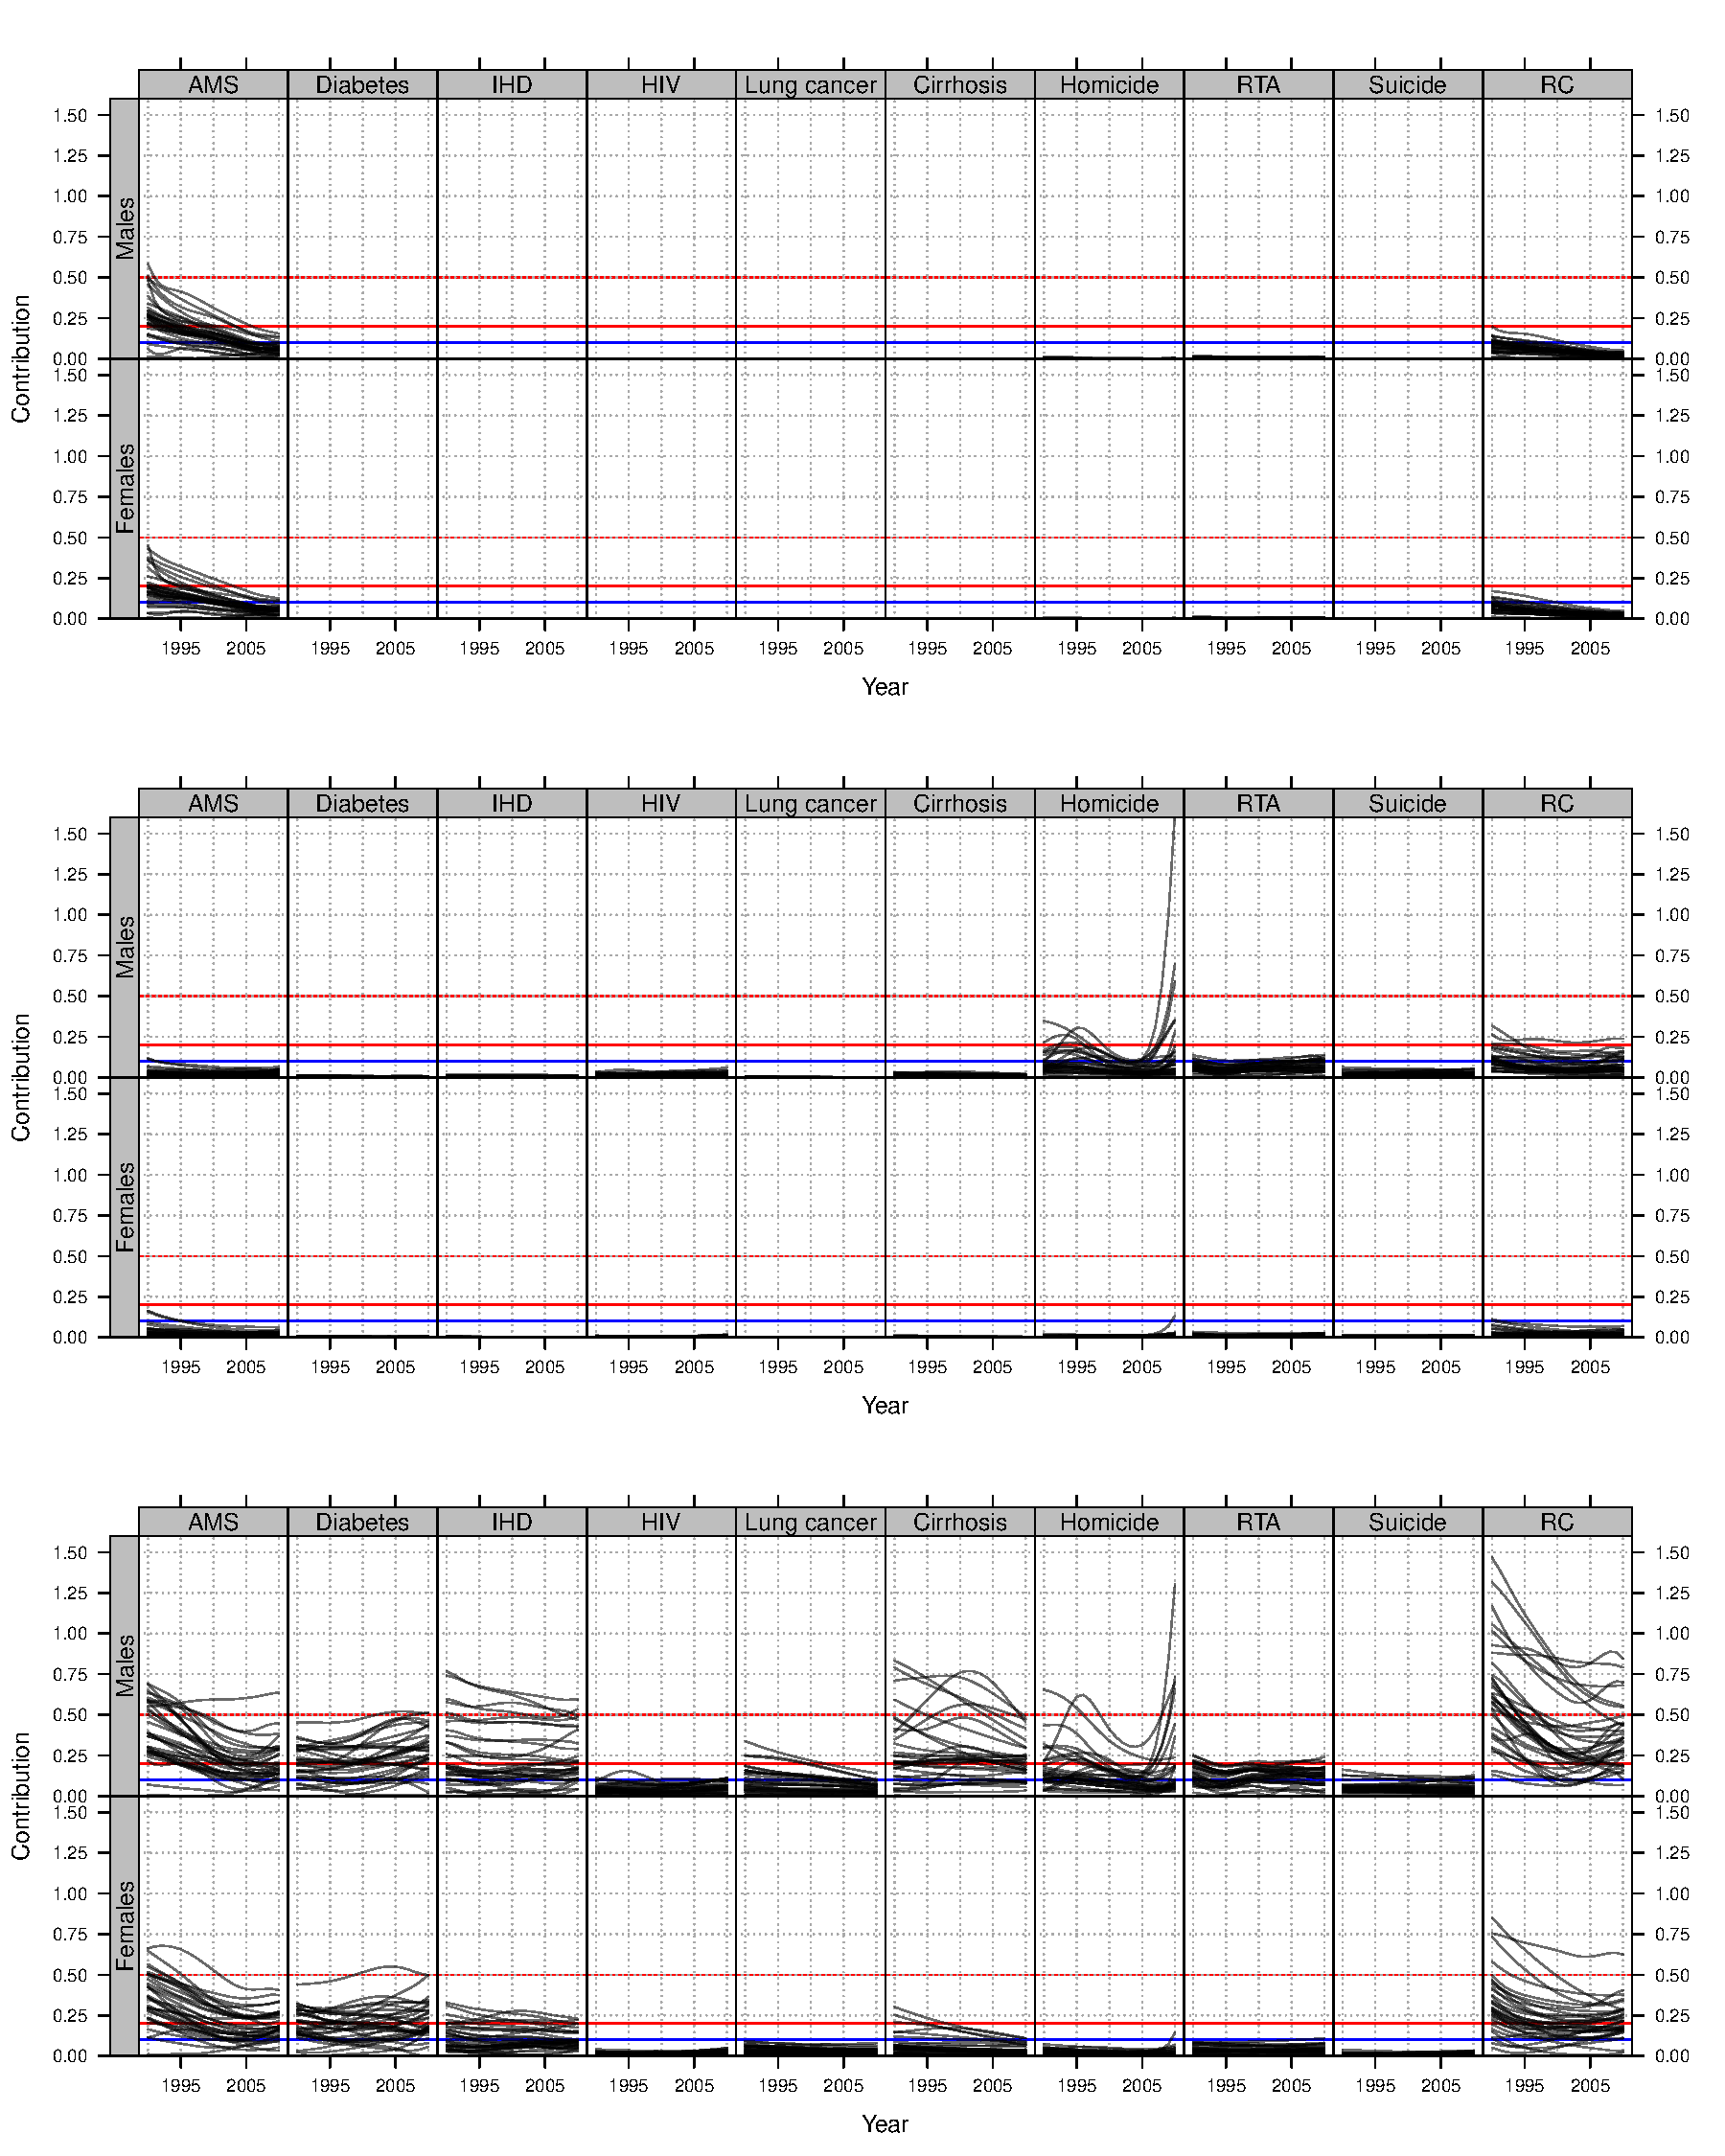
\includegraphics[scale=.5]{Figures/TLE_Decomp.pdf}
Source: own calculations based on INEGI and SOMEDE
\end{figure}

\begin{figure}[\textwidth]
\caption{Homicide-specific contributions to the difference between observed and BP. (preliminar figure)}
\centering
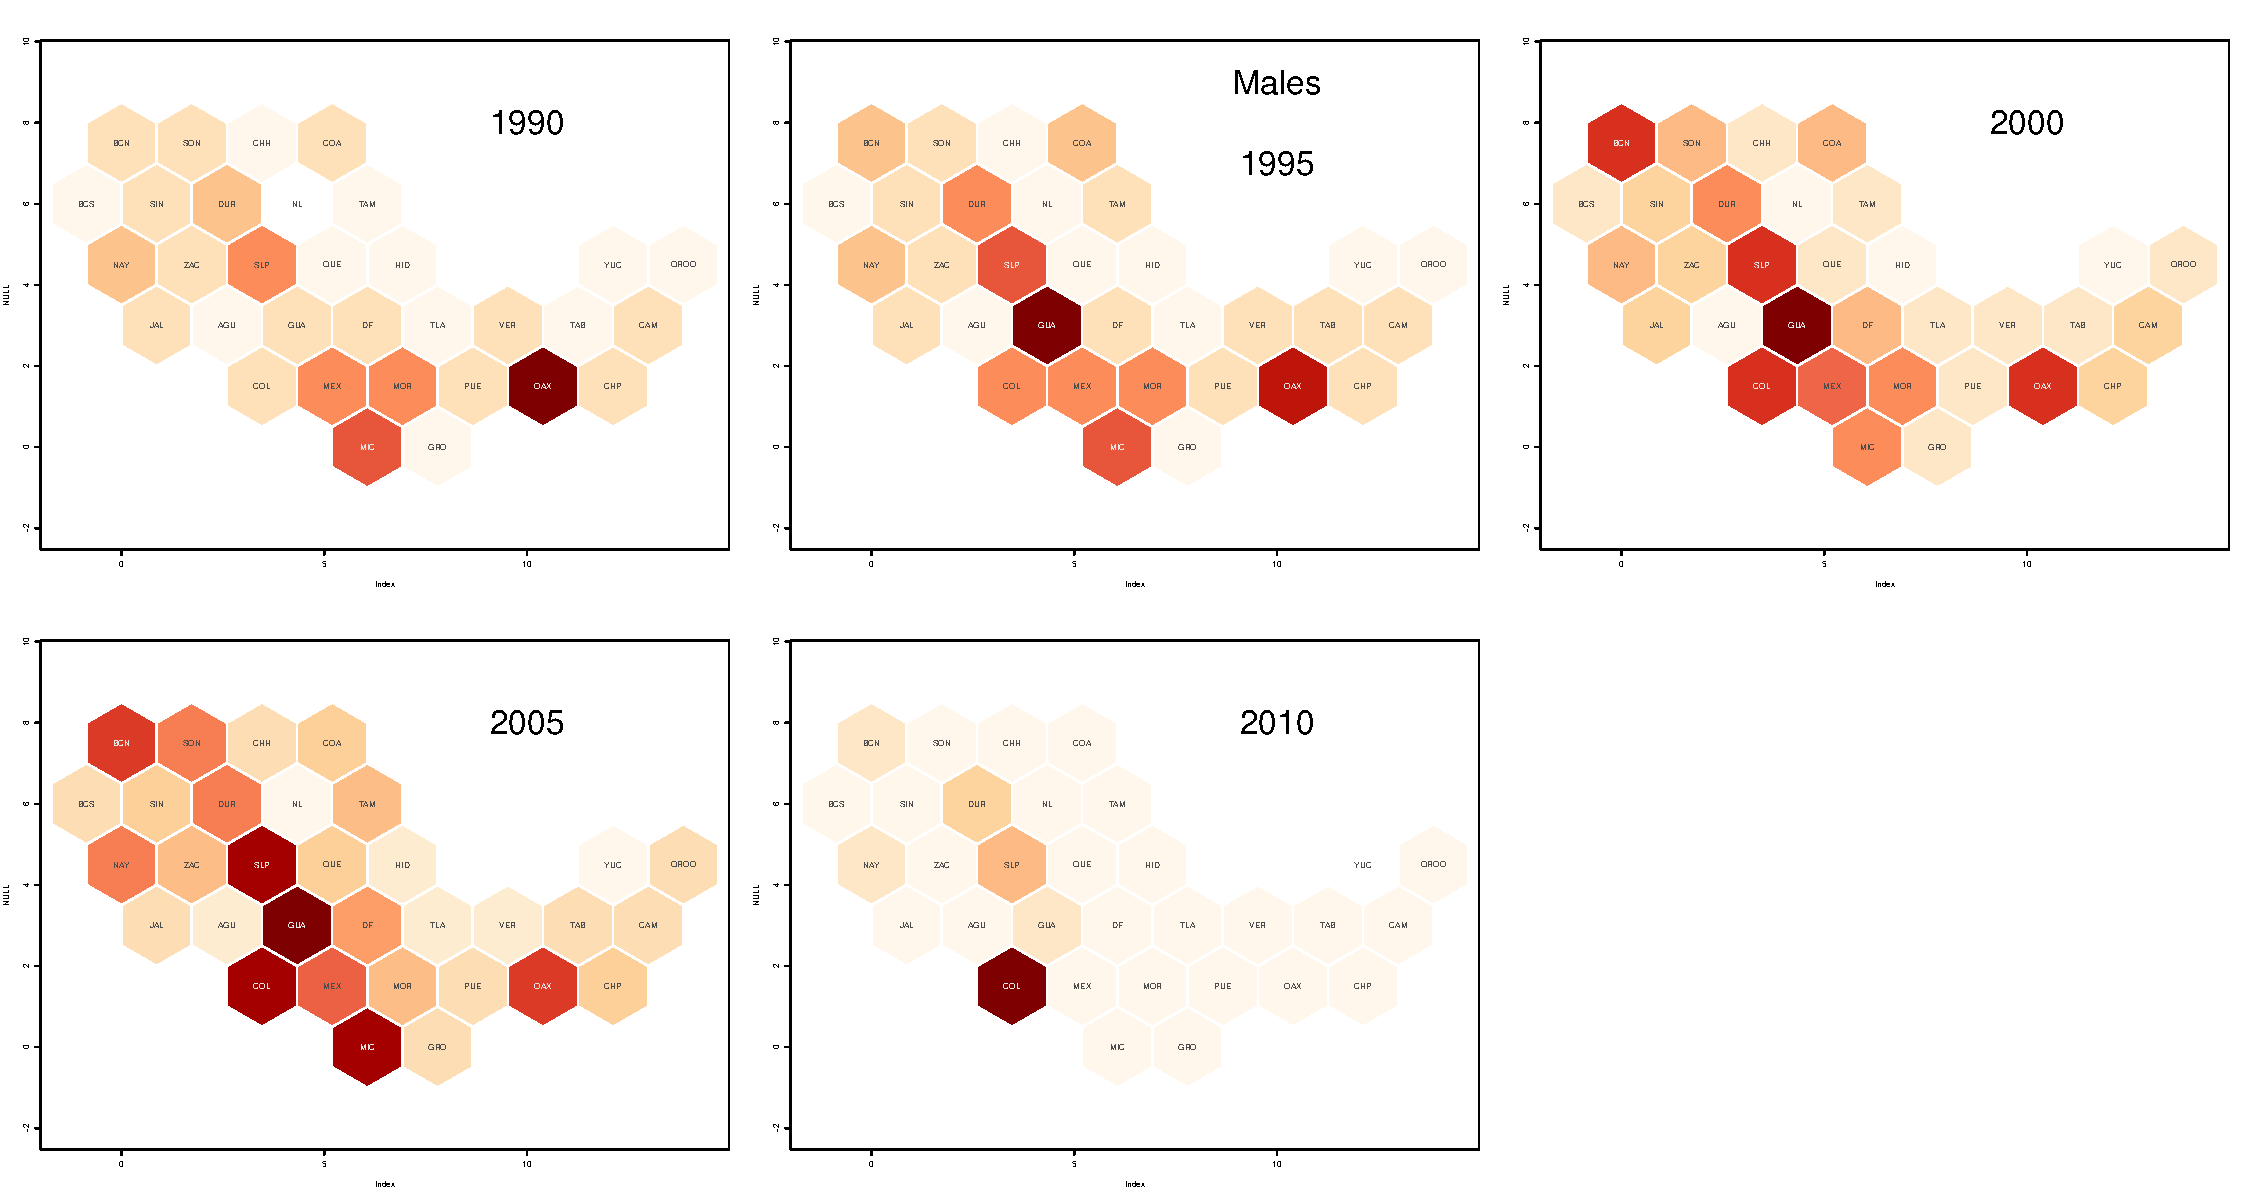
\includegraphics[scale=.4]{Figures/HexMex_maps_homicide.pdf}
Source: own calculations based on INEGI and SOMEDE
\end{figure}


\begin{figure}
\centering
\caption{Deviance from BP caused by Homicide 1990-2010}
\animategraphicsutoplay, controls, scale=.5]{3}{Figures/HexMex_Homicide_15-39}{0}{20}
\end{figure}



%This will show a few small multiples figures, tbd 

%\section*{Discussion}
%Talk about the role of homicide and other major causes. How many years of life
%were lost? (not just expectancy). maybe..

\section*{Discussion}
It is both curious and concerning that the best practices trends have not been
steadily increasing over the period studied. Rather, trends were irregular for
children, flat for adults, and decreasing for older adults. We expected
that the geographic diversity in Mexico would offset the recent mortality
setbacks known from states such as Chihuahua and Durango. If the best practices
trend determines our expectations for future mortality, we can conclude that
our expectations ought to have been stagnant or deflating over time, depending
on the age group considered. It would still represent a great success if
mortality were to drop to the best practices level in all states, as unrealistic as this may seem, but at the same time we expect
the best practices trend to increase given a mix of new technologies, reforms,
and improved material wellbeing.

Despite this pessimistic finding about the best practices trend, all states have
converged toward the best practices temporary life expectancy for the age group
from 0 to 14 over the 21 years studied. This is an important finding to report,
and it could be related to decreases in infectious and respiratory diseases
\citep{canudas2014}, which is consistent with public health
interventions in the period. A forthcoming age-cause decomposition exercise will
shed more light on this point.

Males experienced the same positive trend of convergence in the age group 15 to
39 until the year 2006, when a sudden and sizeable excess in homicide mortality
began in particular states, especially on the Northern border with the U.S.A.
The surge in violent deaths overlapped with a more widespread and earlier
trend in increasing diabetes mortality. It is important to note that the
so-called accident hump grew manifold in size due to violent deaths in
particular states. Here too, our forthcoming decomposition
will shed further light on these observations. Between-state variance in
temporary life expectancy was much smaller for females over the same period,
though females showed the same overall trend of convergence, followed by
divergence after 2006.

For older adults in the 39 to 74 age group, all states except for Chihuahua and
Baja California converged, albeit not toward the best practices trend. Instead,
the best practices trend decreased toward the state trends. Males experienced no
notable improvements in these age groups over the period, while females only
experienced minor improvements, excepting Chihuahua and
Baja California. Of the three age groups considered, the older adult age group
has the most potential for gains in the future. All age groups considered have
room to improve, and many states have much potential for recovery.

%}
%\bibliographystyle{plainnat}
 \bibliography{AburtoRiffe_Bib.bib}

\end{document}


